\documentclass[11pt]{article}
\usepackage{times}
\usepackage{url}
\usepackage{latexsym}
\usepackage{graphicx}
% För svenska tecken åäö
\usepackage[T1]{fontenc}
\usepackage[utf8]{inputenc}
\usepackage{tabularx}
\usepackage[margin=3.4cm]{geometry}
\usepackage{titlesec}
\usepackage{csquotes}
% Created by Hercules Dalianis, December 24, 2019

\usepackage[square,sort,comma,numbers]{natbib}
\usepackage{hyperref} 
%\bibliographystyle{apalike}
\bibliographystyle{vancouver}

% square brackets and comma separator between authors
\setcitestyle{square,comma}

\usepackage{authblk}

\usepackage{abstract}

\title{NLP Enriched Research Data Extracts: An OMOP pipeline for producing structured and unstructured data extracts}
\begin{document}

\renewcommand\Authand{}

\author[1,3]{Kawsar Noor}
\author[1,3]{ Xi Bai}
\author[2]{Adam Sutton}
\author[3]{Baptiste Paul Ribyere}
\author[3]{Tim Roberts}
\author[1,2]{Richard J Dobson}


\affil[1]{University College London, London, United Kingdom}
\affil[2]{King's College London, London, United Kingdom}
\affil[3]{University College London Hospitals, London, United Kingdom}
 
\date{}
\maketitle

% Vänsterjustera abstract heading
\renewcommand{\absnamepos}{flushleft}
\setlength{\absleftindent}{0pt}
\setlength{\absrightindent}{0pt}

\section{Introduction}
The shift towards digitising hospital data in the UK has opened up opportunities for large scale evidence based research due to the faster access to more comprehensive data. Facilitating such research however requires serious considerations of how data can be structured to ensure better of multi-site collaboration, interoperability of data between systems and regulatory compliance. Standardised data models such as the OMOP common data model attempt to address these needs however in practise through such models standardising the free-text portion of the record remains difficult on account of two things: the first is that the free text contains valuable clinical information that requires extraction/structuring and secondly, as per governance requirements, the text needs to be devoid of any personal identifiable patient data (PID). 

In this work we present and end-to-end pipeline and workflow for providing deidentified EHR extracts following the OMOP standard. The pipeline has been developed at UCLH as part of a `data extracts for research service' available within the trust. The pipeline is broadly comprised of two components: a component for populating the structured fields in the OMOP extract, and the components for populating the `NLP/free text' parts of the extract. The `NLP' tables export free-text notes and any extracted medical concepts present in the free text. At UCLH we have deployed AnonCAT and MedCAT for both of these respective tasks. 


\begin{figure}[h]
\centering
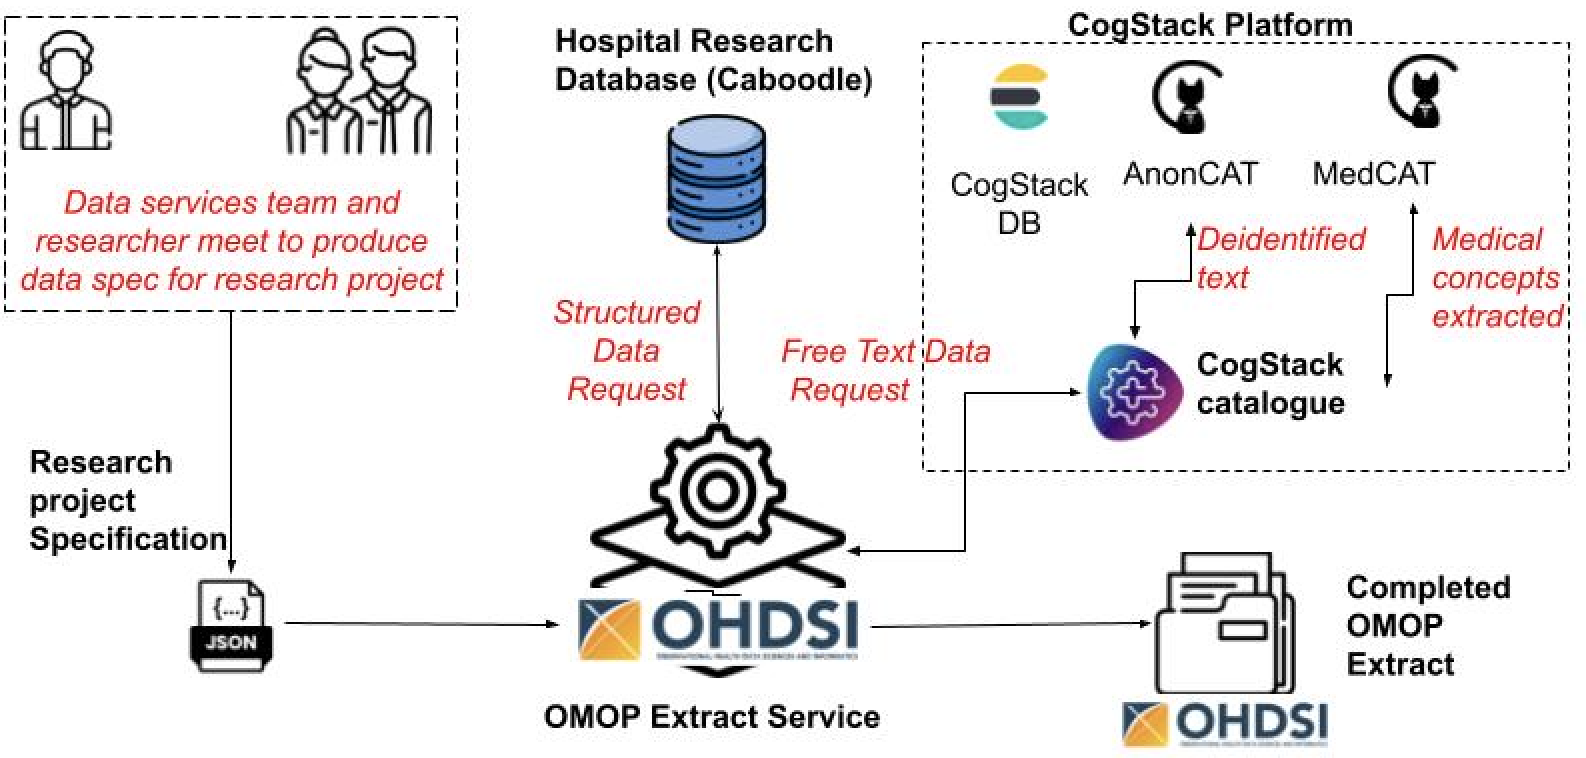
\includegraphics[width=0.8\linewidth]{pipeline.png}
\caption{End-to-end OMOP extraction service.}
\label{pipeline}
\end{figure}



\section{Methods and Data}

Figure \ref{pipeline} depicts the end-to-end OMOP data extract service. The service starts with a consulation between the data extract services team and the researcher which yields a research project specification files describing the required cohort and associated meta data. Following this the specification file is fed to the OMOP extraction service (OMOP ES). OMOP ES subsequently makes two calls. The first is to a hospital managed research database called Caboodle which is used to populate various structured OMOP fields such as demographic data, problem list and meta data about hospital visits etc. 

The second call is to the CogStack platform \cite{cogstack-uclh} for the free-text data. OMOP ES communicates with the platform via the CogStack catalogue application through which it specifies the various types of notes it requires and concepts it wants extracted. The catalogue application subsequently retrieves the free text and passes it through the UCLH trained and hosted AnonCAT service \cite{10337202} for deidentidcation. MedCAT for clinical concept extraction. The data is subsequently fed back to the OMOP ES for populating the NLP tables.

One the main challenges with this pipeline is validating the quality of deidenfitied data. UCLH have imposed a number of guidelines to address this including requiring the original requester to spot-check a subset of the documents. Secondly every, as a seperate process, every six months an approved annotator acts as a motivated intruder and test the model using a combination of synthetic data and real data. Using these mechanisms the AnonCAT model is able to benefit from the feedback which goes onto furhter improving the model during the next cycle of training. 

\section{Results}
To date the OMOP ES pipeline has been used to supply mostly structured data however as of this year there increased demands for data extracts with free text including a collaboration with multiple sclerosis \cite{pinpoint}. 

\section{Conclusion}
We have demonstrated the feasibility of deploying an end-to-end research data extract service for providing OMOP-ified extracts. The pipeline has several dependencies including those to the NLP services AnonCAT and MedCAT.

\section{Study context}
The OMOP ES and CogStack integration work was a collaboration between UCLH and KCH. Additional the AnonCAT model was cross trained between KCH and UCLH.


\bibliography{template-references.bib}
\end{document}
